\newpage
\section{Конструкторская часть}

Рассмотрим стандартный алгоритм умножения матриц, алгоритм Винограда и улучшенный
алгоритм Винограда.

\subsection{Функциональная модель}

На рисунке \ref{img:idef0} представлена функциональная модель IDEF0 уровня 1.

\begin{figure}[H]
    \center{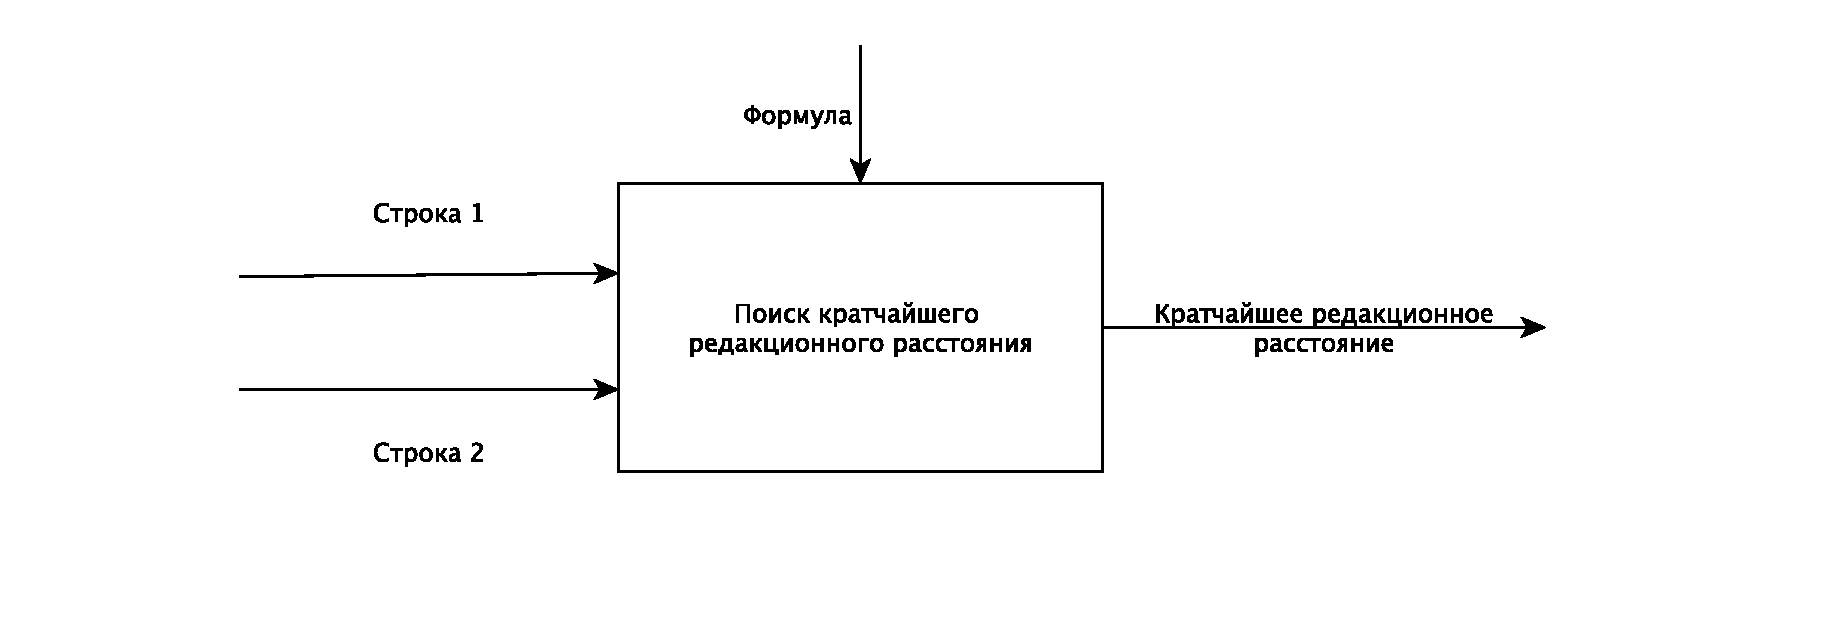
\includegraphics[scale=0.8]{IDEF0}}
    \caption{Функциональная модель IDEF0 уровня 1}
    \label{img:idef0}
\end{figure}

\subsection{Схемы алгоритмов}

На рисунке \ref{img:default} изображена схема стандартного алгоритма произведения
матриц

\begin{figure}[H]
    \center{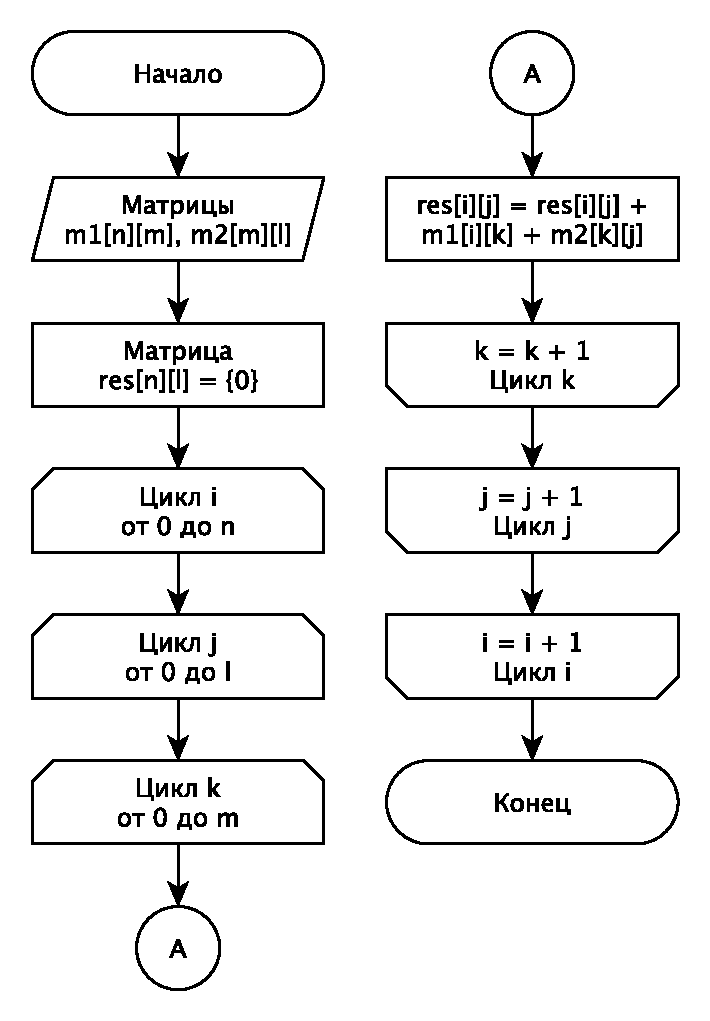
\includegraphics[scale=0.65]{default}}
    \caption{Схема стандартного алгоритма}
    \label{img:default}
\end{figure}

На рисунке \ref{img:vinograd} изображена схема алгоритма
Винограда произведения матриц

\begin{figure}[H]
    \center{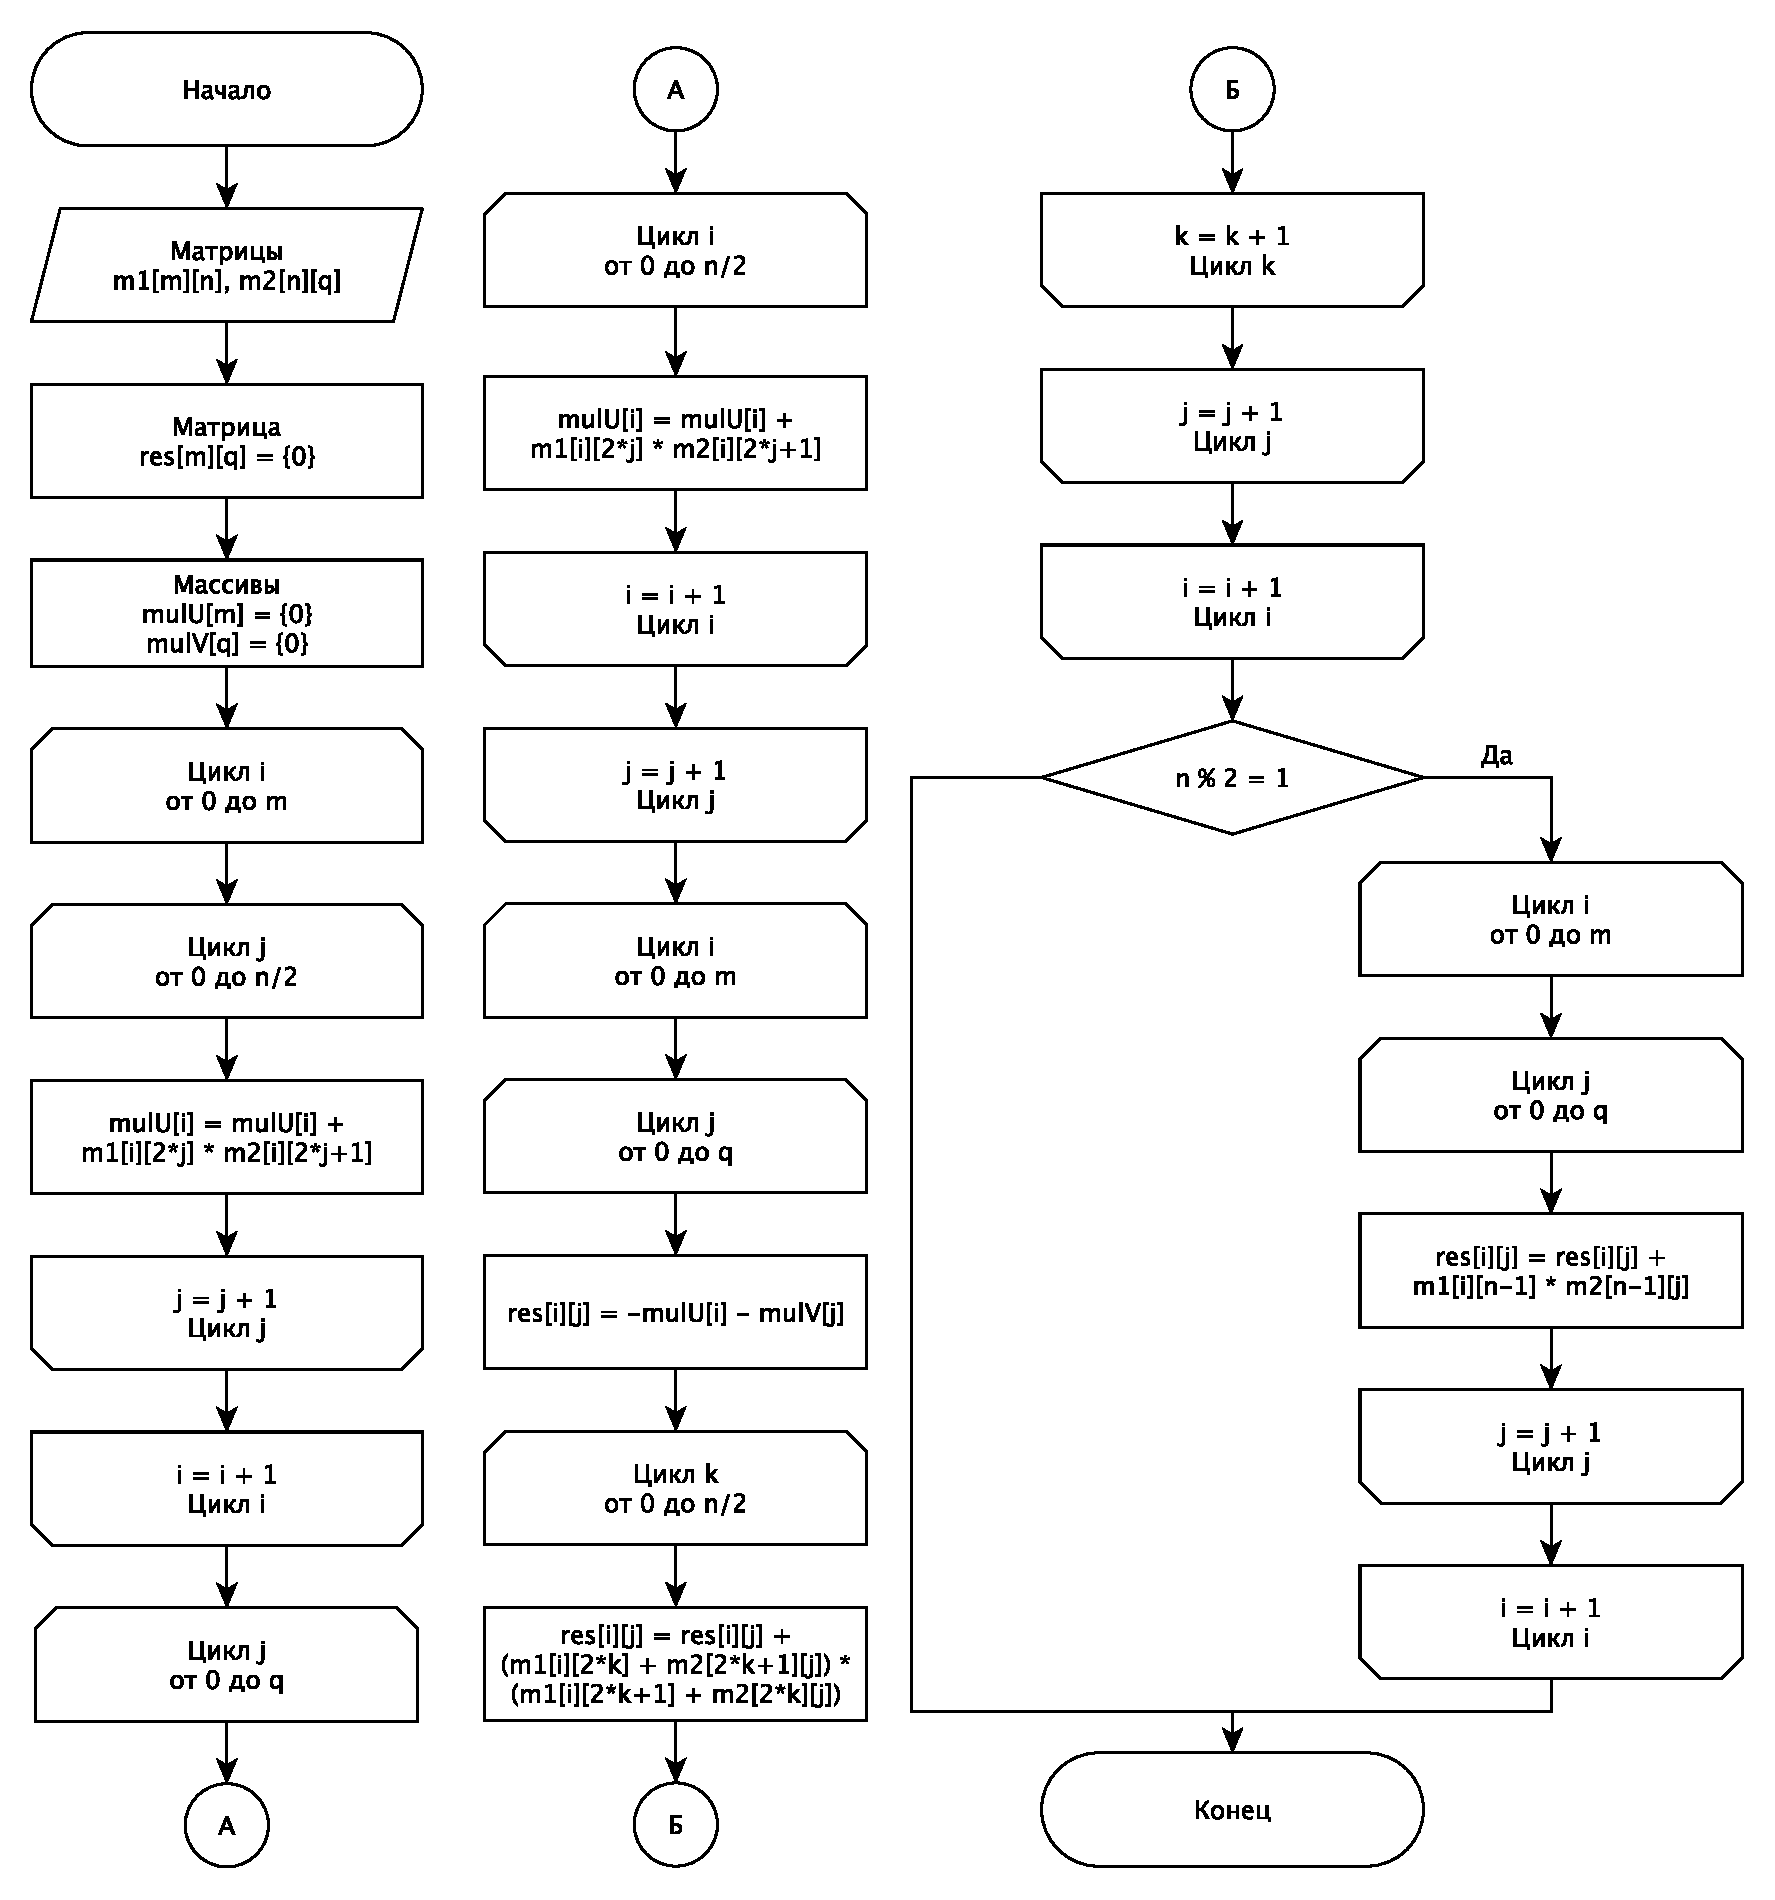
\includegraphics[scale=0.6]{vinograd}}
    \caption{Схема алгоритма Винограда}
    \label{img:vinograd}
\end{figure}

На рисунке \ref{img:modvinograd} изображена схема
оптимизированного алгоритма Винограда. Его удалось оптимизировать в трех местах:

\begin{itemize}
    \item {\ttfamily mulU} и {\ttfamily mulV} сразу ищутся с отрицательным знаком;
    \item для прибавления выражений к переменной используется оператор {\ttfamily +=};
    \item вместо цикла до $\frac{n}{2}$ происходит прибавление к переменной цикла
        по 2, а не по 1.
\end{itemize}

\begin{figure}[H]
    \center{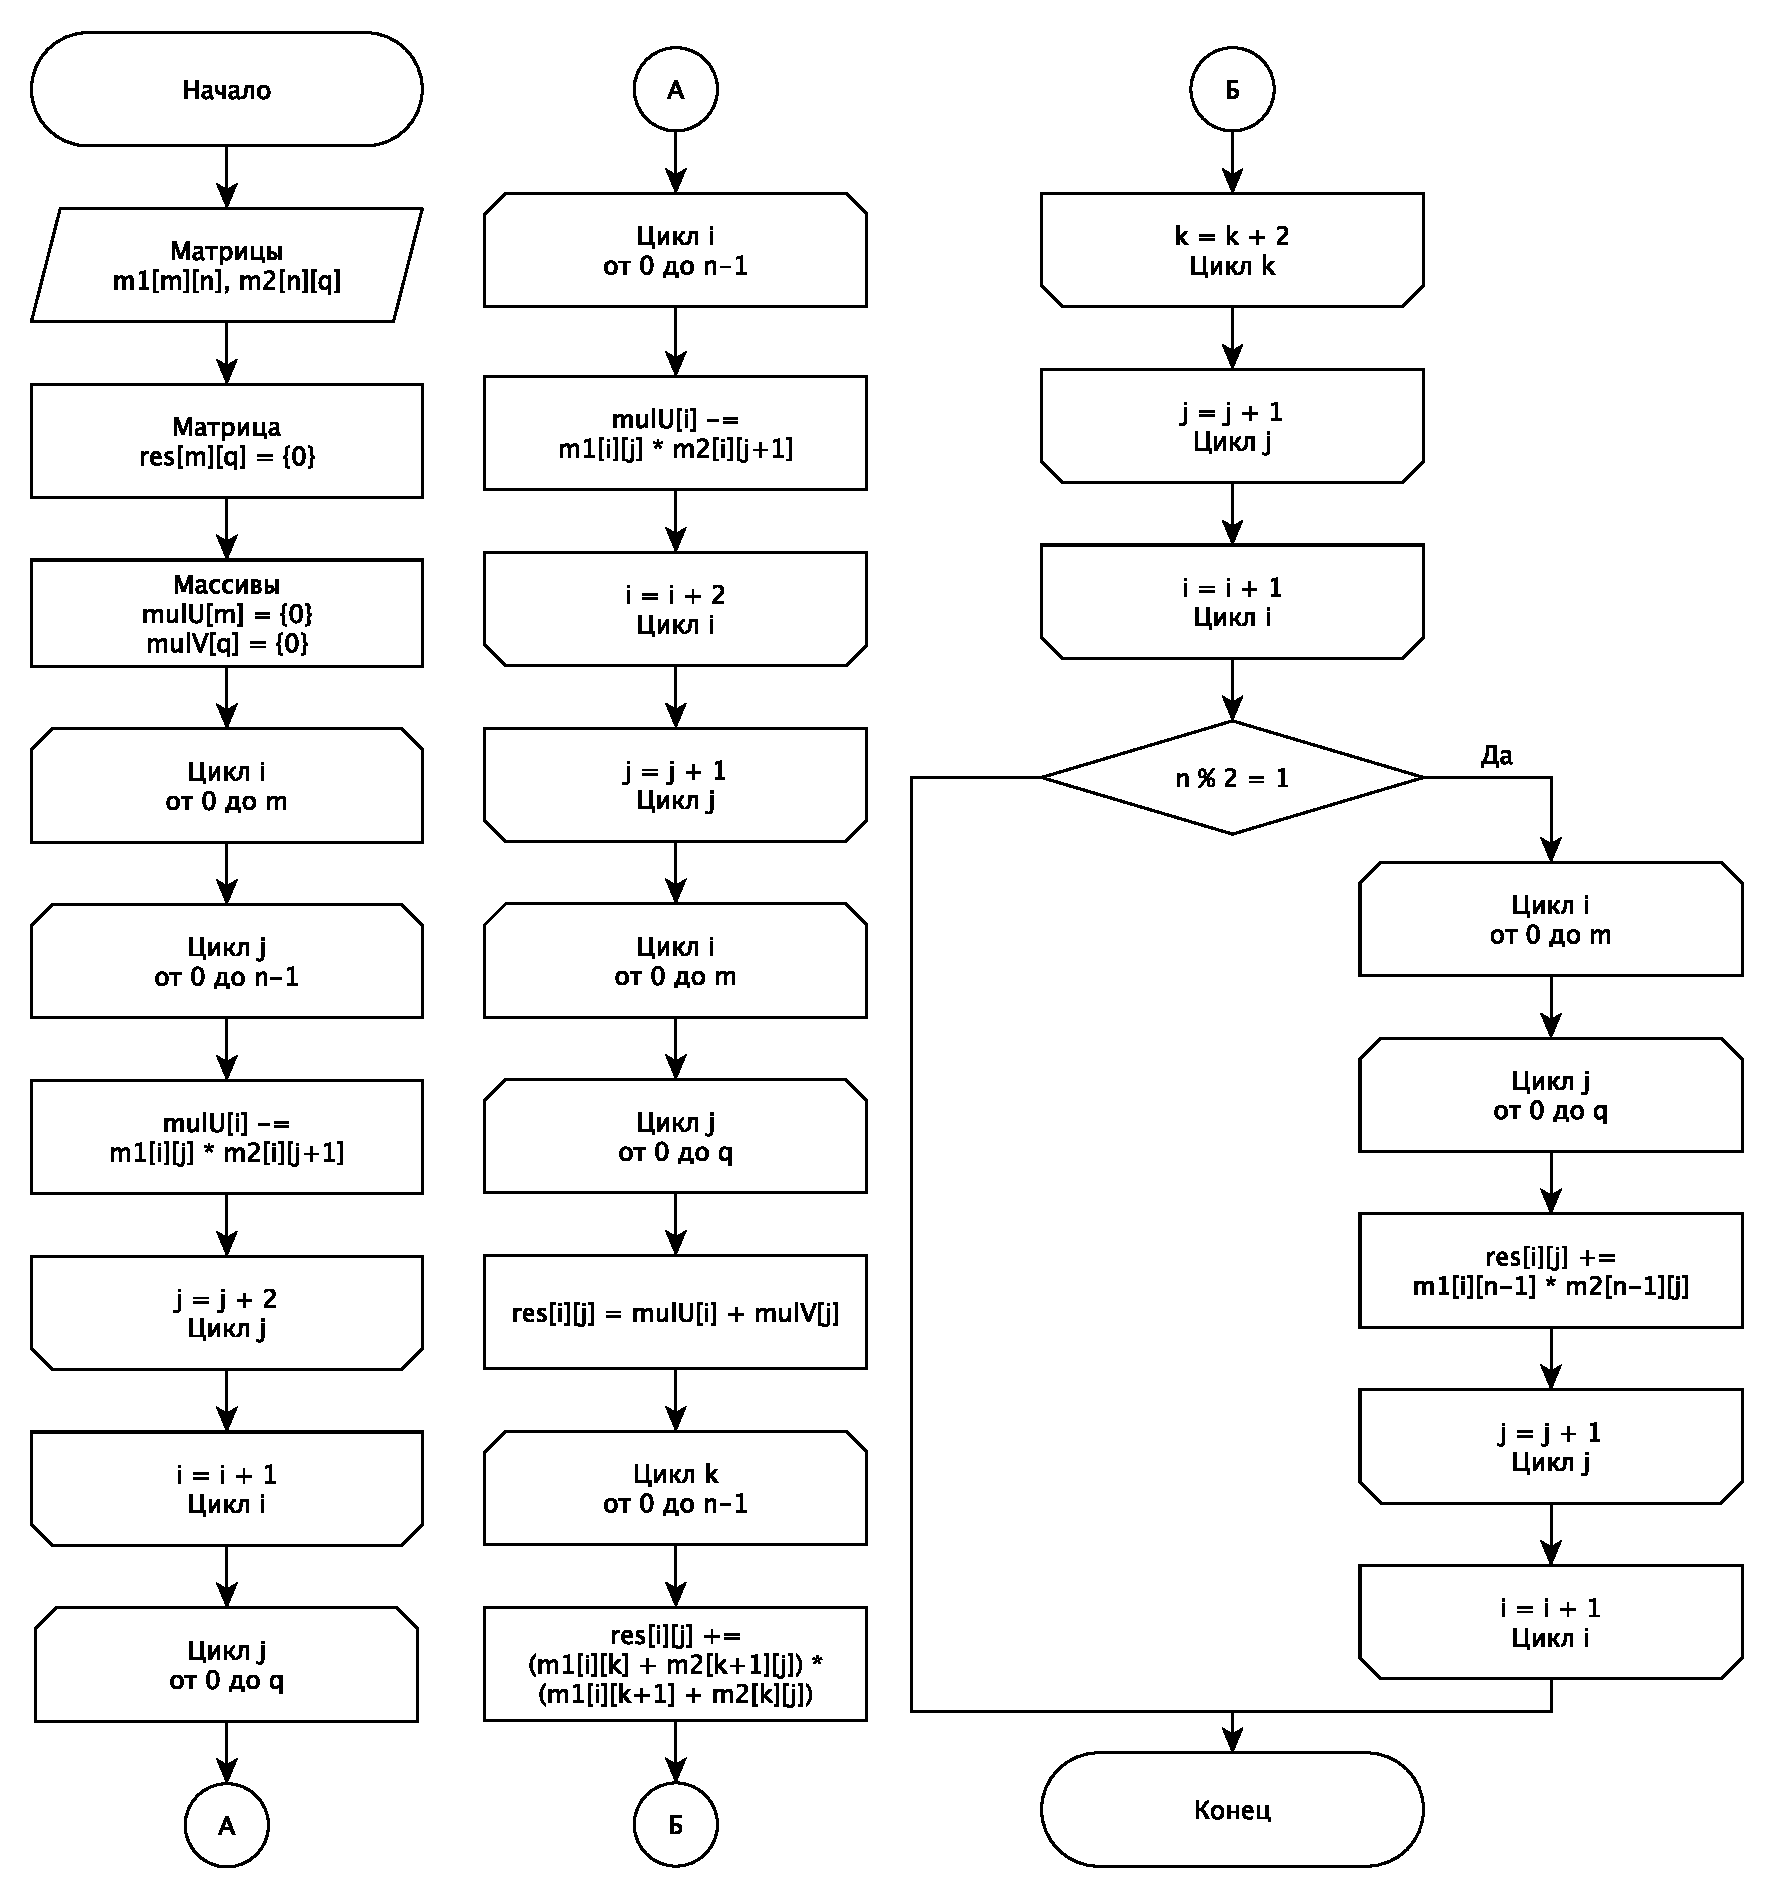
\includegraphics[scale=0.6]{modvinograd}}
    \caption{Схема оптимизированного алгоритма Винограда}
    \label{img:modvinograd}
\end{figure}

Произведем теоретическую оценку трудоемкости алгоритмов умножения матриц

\begin{enumerate}
    \item Стандартный алгоритм

        \begin{equation}
            f = 2 + M(2 + 2 + Q(2 + 2 + N(2 + 8 + 1 + 1 + 1))) =
            13MNQ + 4MQ + 4M + 2
        \end{equation}

    \item Алгоритм Винограда

        \begin{equation}
            f = 2 + M(2 + 2 + Q(2 + 4 + 3 + 3 + \frac{N}{2}(3 + 12 + 11))) =
            13MNQ + 12MQ + 4M + 2
        \end{equation}

        Но доля умножения меньше, чем в стандартном.

    \item Алгоритм Винограда с оптимизацией

        После введенных оптимизаций трудоемкость будет в формуле \ref{modvineff}.

        \begin{equation}\label{modvineff}
            f = 2 + M(2 + 2 + Q(2 + 6 + 2 + \frac{N}{2}(2 + 3 + 7 + 6))) =
            9MNQ + 10MQ + 4M + 2
        \end{equation}
\end{enumerate}

\subsection{Выводы}

За счет уменьшения доли умножения алгоритм Винограда теоретически будет работать быстрее,
чем обычный, но его удалось оптимизировать, уменьшив количество операций до числа,
меньшего, чем у стандартного алгоритма. Проверим данные предположения на реализованных
алгоритмах.
